\chapter{Integrands with antiderivate discontinuities in their Integral bounds}
\label{chap:3}

In this chapter, we will show how some functions suffer from the issues mentioned in \autoref{chap:2}. For this purpose, we just need to find $g(x)$ which are discontinuous and can create our integrands by working our way up from there.

\section{First example}
It is easy to see that the function $g(x) = 1/(x-1)^3$ is discontinuous at the point $x=1$. \autoref{F2a} shows this with clarity.
\begin{figure}[h]
	\centering
	\begin{subfigure}[t]{0.49\textwidth}
		\centering
		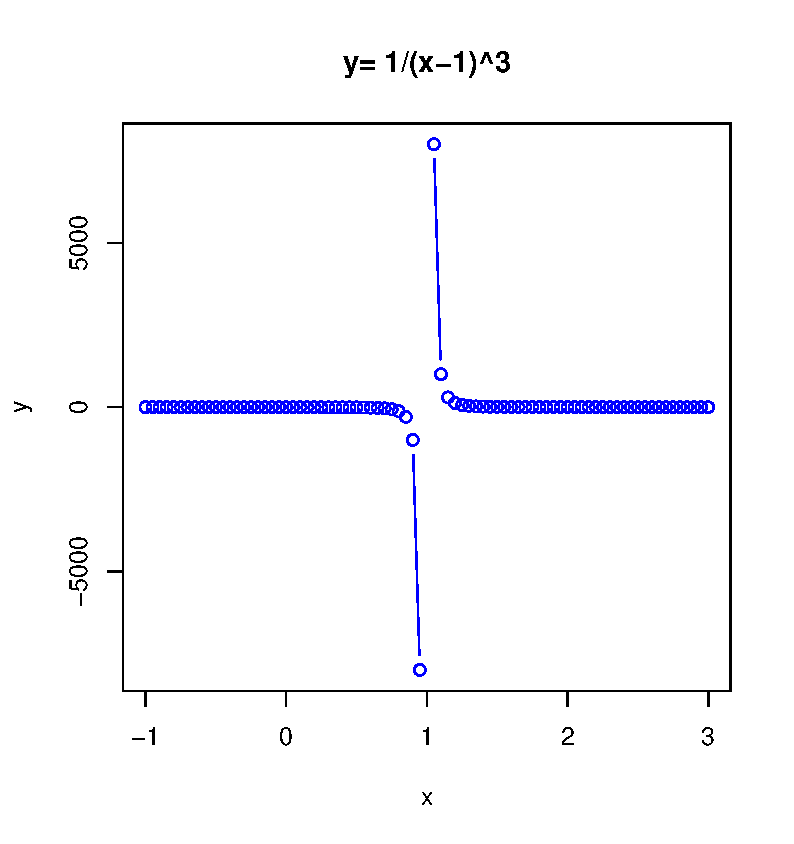
\includegraphics[width=\linewidth]{Plot2a.pdf}
		\phantomsubcaption
		\label{F2a}
	\end{subfigure}
	\hfill
	\begin{subfigure}[t]{0.49\textwidth}
		\centering
		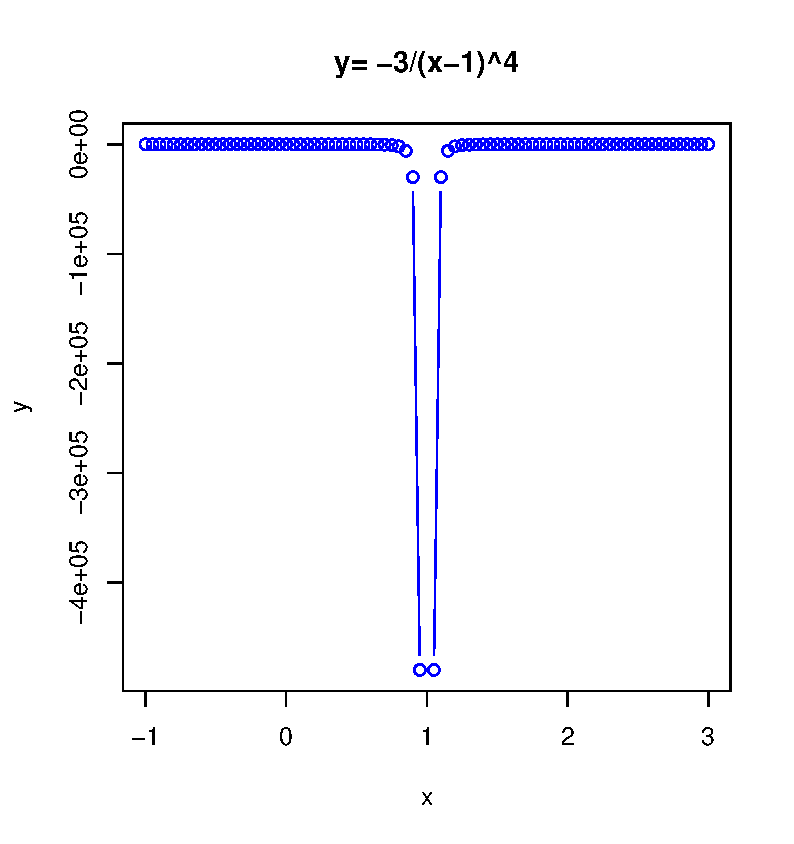
\includegraphics[width=\linewidth]{Plot2b.pdf}
		\phantomsubcaption
		\label{F2b}
	\end{subfigure}
	\caption{(a)Plot of $y=1/(x-1)^3$ generated using R. (b)Plot of $y = -3/(x-1)^4$ generated using R.}\label{F2}
\end{figure}
It's easy to see that the derivative $\mathrm{d}g(x)/\mathrm{d}x = -3/(x-1)^4$ is shown in \autoref{F2b} and does not have a discontinuity at that point, but it can be checked that the integral would be infinite.
Consider the integral $I$ shown below $$I = \int_{0}^{2}\frac{\mathrm{d}x}{(x - 1)^4}$$
Using the direct antiderivate method we get
$$I = \int_{0}^{2}\frac{1}{(x-1)^4}\,\mathrm{d}x = -\frac{1}{3}\frac{1}{(x-1)^3}\bigg\rvert_{0}^{2} = -\frac{2}{3}$$
Now, breaking it up into it constituents as shown below
\begin{align*}
	I &= \int_{0}^{2}\frac{1}{(x-1)^4}\,\mathrm{d}x = \int_{0}^{1^-}\frac{1}{(x-1)^4}\,\mathrm{d}x + \int_{1^+}^{2}\frac{1}{(x-1)^4}\,\mathrm{d}x \\
	&=\frac{1}{3}\frac{1}{(x-1)^3}\bigg\rvert_{1^-}^{0} + \frac{1}{3}\frac{1}{(x-1)^3}\bigg\rvert_{2}^{1^+} \\
	& \to \infty &&
\end{align*}

\section{Second example}

Another example of a discontinuous $g(x)$ is $\tan(x)$ such that $x \in (0, \pi)$.

\begin{figure}[h]
	\centering
	\begin{subfigure}[t]{0.49\textwidth}
		\centering
		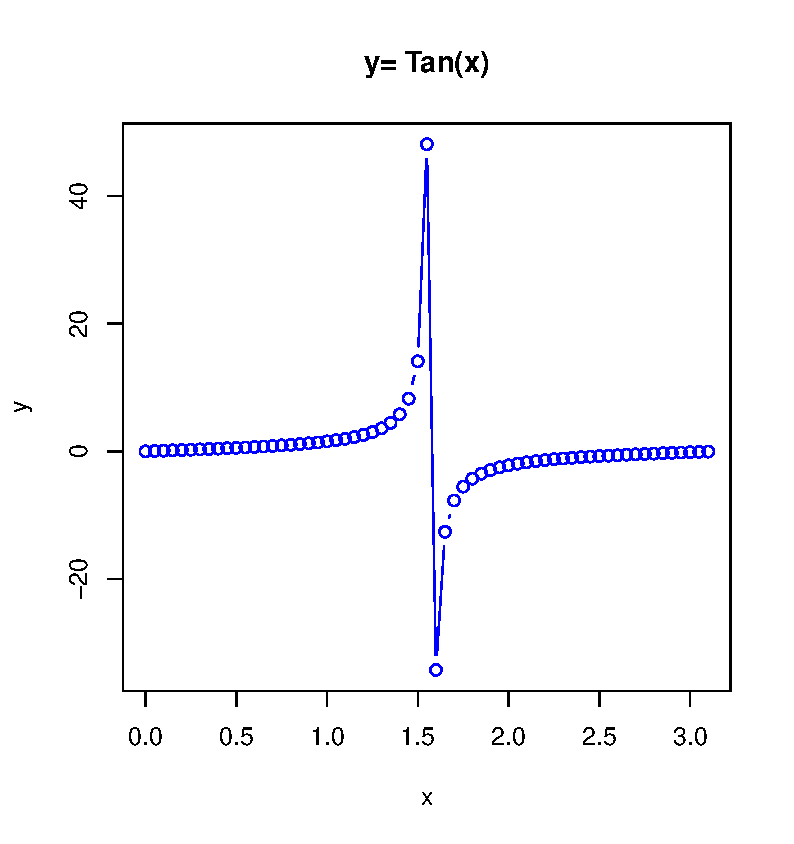
\includegraphics[width=\linewidth]{Plot3a.pdf}
		\phantomsubcaption
		\label{F3a}
	\end{subfigure}
	\hfill
	\begin{subfigure}[t]{0.49\textwidth}
		\centering
		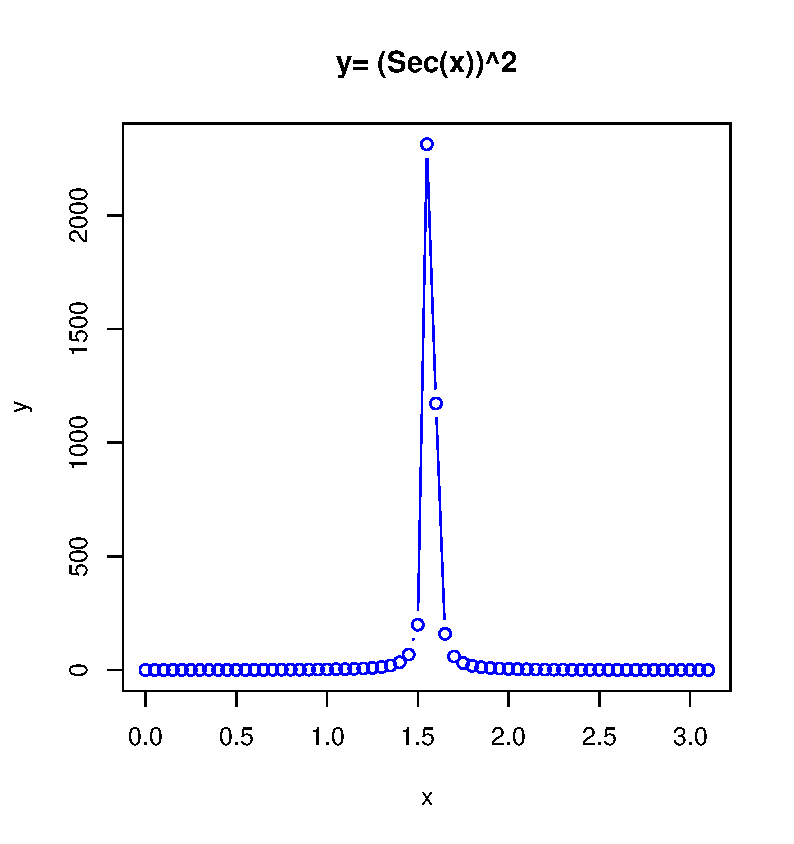
\includegraphics[width=\linewidth]{Plot3b.pdf}
		\phantomsubcaption
		\label{F3b}
	\end{subfigure}
	\caption{(a)Plot of $y=\tan{x}$ generated using R. (b)Plot of $y = (\sec{x})^2$ generated using R.}\label{F3}
\end{figure}

The discontinuity in \autoref{F3a} can be seen at $x =\pi/2$ for $g(x) = \tan{x}$. Thus, the consequence of directly using the antiderivative method for the problem can be seen below and yields a value of zero which is incorrect and can be directly judged from \autoref{F3b}.

\begin{align*}
	I &= \int_{0}^{\pi}\sec^2{x}\,\mathrm{d}x \\
	&= \tan{x}\bigg\rvert_{0}^{\pi} \\
	&= 0
\end{align*}

However, splitting it up into integrals on either side of $\pi/2$ yields the infinitely large area as shown below.

\begin{align*}
	I = \int_{0}^{\pi}\sec^2{x}\,\mathrm{d}x &= \int_{0}^{{\frac{\pi}{2}}^-}\sec^2{x}\,\mathrm{d}x + \int_{{\frac{\pi}{2}}^+}^{\pi}\sec^2{x}\,\mathrm{d}x \\
	&= \tan{x}\bigg\rvert_{0}^{{\frac{\pi}{2}}^-} + \tan{x}\bigg\rvert_{{\frac{\pi}{2}}^+}^{\pi} \\
	& \to \infty
\end{align*}